% Template for PLoS
% Version 1.0 January 2009
%
% To compile to pdf, run:
% latex plos.template
% bibtex plos.template
% latex plos.template
% latex plos.template
% dvipdf plos.template

\documentclass[10pt]{article}

% amsmath package, useful for mathematical formulas
\usepackage{amsmath}
% amssymb package, useful for mathematical symbols
\usepackage{amssymb}

% graphicx package, useful for including eps and pdf graphics
% include graphics with the command \includegraphics
\usepackage{graphicx}

% cite package, to clean up citations in the main text. Do not remove.
\usepackage{cite}

\usepackage{color} 

% Use doublespacing - comment out for single spacing
\usepackage{setspace} 
\doublespacing

\usepackage{multirow}

% Text layout
\topmargin 0.0cm
\oddsidemargin 0.5cm
\evensidemargin 0.5cm
\textwidth 16cm 
\textheight 21cm

% Bold the 'Figure #' in the caption and separate it with a period
% Captions will be left justified
\usepackage[labelfont=bf,labelsep=period,justification=raggedright]{caption}

% Use the PLoS provided bibtex style
\bibliographystyle{plos2009}

% Remove brackets from numbering in List of References
\makeatletter
\renewcommand{\@biblabel}[1]{\quad#1.}
\makeatother


% Leave date blank
\date{}

\pagestyle{myheadings}
%% ** EDIT HERE **


%% ** EDIT HERE **
%% PLEASE INCLUDE ALL MACROS BELOW

%% END MACROS SECTION

\begin{document}

% Title must be 150 characters or less
\begin{flushleft}
{\Large
\textbf{RNA-Seq Assembly Discovers Many Splice Variants}
}
% Insert Author names, affiliations and corresponding author email.
\\
Likit Preeyanon$^{1}$, 
Jerry B. Dodgson$^{1}$
Hans Cheng$^{2}$, 
C. Titus Brown$^{3,1 \ast}$
\\
\bf{1} Microbiology and Molecular Genetics, Michigan State University, East Lansing, MI, USA.
\\
\bf{2} Avian Disease and Oncology Laboratory, East Lansing, MI, USA.
\\
\bf{3} Department of Computer Science and Engineering, Michigan State University, East Lansing, MI, USA.
\\
$\ast$ E-mail: ctb@msu.edu
\end{flushleft}

% Please keep the abstract between 250 and 300 words
\section*{Abstract}
Comparison of spliced reads and reference gene annotations has been successfully used to discover alternative
splicing in model organisms. However, the method cannot be applied in organisms without high-quality reference genome and
gene annotations. In this article, we introduce a pipeline, based on \emph{de novo} assembly, that constructs gene models with splice
variants.
The pipeline includes a new technique called local assembly that enhances the sensitivity of
alternative splicing detection.
We demonstrates that the pipeline detects many novel splice variants in RNA-Seq data from chicken spleens.
Some of those splice variants; however, only detected by our pipeline and not Cufflinks.
This indicates that the pipeline can be used to facilitate splice variants detection from RNA-Seq.
% Please keep the Author Summary between 150 and 200 words
% Use first person. PLoS ONE authors please skip this step. 
% Author Summary not valid for PLoS ONE submissions.   
\section*{Author Summary}

\section*{Introduction}
Until recently, studies of alternative splicing had been limited to a small
number of genes and isoforms due to high-cost and low-throughput sequencing
of expressed sequence tags (ESTs) and full-length cDNA libraries.  
RNA sequencing (RNA-Seq) using the next-generation sequencing (NGS) has been
used successfully in many studies to gain unprecedented insight into a
complexity of transcriptomes.
It has been estimated that, in human, $92-94$\% of multiexon genes undergo alternative
splicing and different isoforms are expressed in different tissues\cite{Wang:2008ea}.
This suggests that even in human a large number of splice variants have not been explored.

%Since sequences from RNA-Seq (reads) are very short (~50--250bp for Illumina reads),
%it is nokt feasible to assess expression isoforms and their structures without mapping reads
%to a reference annotation or reconstructing a full-length transcript from short reads.

Despite the small size of sequencing reads, several studies have detected
novel splice junctions based on alignment of reads spanning across putative exon junctions.
To map reads across exon junctions, reads are split into two parts and each part is mapped
to the genome independently.
A splice junction is then identified based on alignments of each half of a read
that fall between two exons at exon-intron boundaries.
With this approach, Wang \emph{et al} have identified a large number of
splice junctions that are not annotated from human cell lines (HUVEC and NHEK)\cite{Wang:2011jq}.
These novel splice sites include both canonical and non-canonical splice sites.
Approximately, $46\%-75\%$ of canonical splice sites are supported by ESTs.
Novel splice junctions have different levels of read coverage suggesting that both high-
and low-expressed isoforms are unannotated.

Using a similar approach, Pickrell \emph{et al} identified more than 150,000 novel canonical splice junctions
in lymphoblastoid cells.
The study also shows that the number of unannotated splice junctions varies among cells from
different human tissues, which suggests tissue-specific expression of isoforms\cite{Pickrell:2010gt}.
A majority of unannotated isoforms found in both studies are from alternative splicing
of annotated exons. Only a small fraction of isoforms contain exons from intergenic or
intronic region.

Several tools have been developed not only to detect novel splice junctions but also to reconstruct
full-length isoforms from short reads without using gene annotations.
These tools are especially useful for transcriptome analysis of organims with poor gene annotations.
Cufflinks\cite{Trapnell:2010kd} relies on splice junctions detected from Tophat\cite{Trapnell:2009dp},
a read aligner that can align reads across putative exon junctions, to reconstruct a full-length transcript.
Cufflinks identified 12,712 novel isoforms, of which 7,395 ($58\%$) contain novel splice junctions in
mouse myoblast cell lines.
Guttman \emph{et al} used Scripture, a tool employing similar mapping-based approach, to reconstruct
a full-length transcripts from mouse RNA-Seq data and discovered approximately 490 novel alternative
isoforms in lincRNA loci, which are expressed in any of the three different cell types\cite{Guttman:2010io}.

Although the mapping-based method has been useful in both detecting splice junctions and isoforms,
it relies heavily on a reference genome.
Hence, organisms lacking a genome or a high-quality one may not find this approach practical.
This limitation can be overcome by \emph{de novo} assembly of short reads.

A number of \emph{de novo} assemblers have been used to reconstruct transcripts from RNA-Seq data in
many studies.
Trinity\cite{Grabherr:2011jb}, was successfully used to reconstruct transcripts from yeast and mouse datasets.
It was also shown that Trinity detects a unique set of novel splice junctions not detected by Cufflinks
or Scripture.
This suggests that \emph{de novo} assembly approach is capabale of increasing sensitivity of detecting
alternative isoforms of a mapping-based method.
Trans-Abyss\cite{Robertson:2010ih} and Oases\cite{Schulz:2012je} are an extension
of Abyss\cite{Simpson:2009iv} and Velvet\cite{Zerbino:2008vu,Zerbino:2009jp} genome assembler
that are tuned to work with RNA-Seq data.
These assemblers are comparable at reconstructing existing and novel alternative isoforms with a slightly
different sensitivity and specificity.
However, Oases with Oases-M has been shown to be superior than other \emph{de novo}
assemblers at discovering isoforms in human and mouse\cite{Schulz:2012je}.

In this study, we present a pipeline that uses Velvet and Oases assembler to
reconstruct alternative isoforms in RNA-Seq data from chickens.
We use a new technique called a local assembly that enhances sensitivity of
alternative isoform detection of Oases.
The results show that the pipeline can detect more isoforms than Oases-M and
can detect isoforms not found by Cufflinks.
We also showed that transcripts reconstructed from \emph{de novo} assembly and mapping-based approach can be
merged to build more complete predicted gene models.

% Results and Discussion can be combined.
\section*{Results}

\subsection*{Local Assembly Enhances Isoform Detection}

We used the Velvet\cite{Zerbino:2008vu} and Oases\cite{Schulz:2012je}
assemblers to construct transcript fragments from four entire Illumina
GAII mRNAseq data sets sequenced from chicken spleen (see Methods and
Materials).  In the assembly, we used multiple distinct k-mer values
for Velvet to sensitively recover as many different isoforms as possible
\cite{Schulz:2012je}.  We chose k-mers between 21 and 31,
and recovered between 340,000 and 370,000 unique sequences from
each data set (see Table~\ref{unique_sequences}, and Materials and
Methods).  These unique sequences represented an unknown number of
true genes, due to fragmentation from low coverage and incomplete
assembly.

We next used Tophat to align mRNAseq reads to the genome and partition
reads by chromosome; we then assembled the partitioned reads with
Velvet and Oases using the same range of parameters as the global
assembly, above.  While the local assemblies were considerably more
computationally efficient, they lacked several thousand unique regions
that were present in the global assembly
% @CTB why are the global ones not included in the final gene models?
(Table~\ref{unique_sequences_matched_mouse}); this is probably due to
the incomplete nature of the current chicken genome assembly, which is
lacking approximately 5\% of its true gene content (cite).
Interestingly, over a hundred regions were present {\em only} in the
local assemblies, suggesting that the local assemblies might be
recovering additional exons.  Significant numbers of unique regions
from both global and local assemblies showed homology to the mouse
genome, indicating that at least some of these unique sequences
represented real sequence content.  Figure~\ref{global_vs_local} shows
an example of different isoforms detected by the two assembly methods.

% @CTB how many reads are discarded in the process of mapping?
% @CTB what does local assembly actually do to the DBG??
% @CTB what happens if you ask how many unique regions there are not
%   represented in the final gene models?

% @CTB DISCSUSS the use of splice junctions for validity; transition
% from transcripts to splice junctions.

\subsection*{Oases-M discards splice variants}

The above approaches recovered transcript fragments, but not entire genes
(figure in suppl?)
To construct a more comprehensive gene set containing all of the
assembled contigs, we tried using Oases-M to merge the assemblies from
multiple $k$ values \cite{Schulz:2012je}.  While it has been
demonstrated that merged transcripts from multiple-k assemblies
contain more isoforms than those from any single $k$, the sensitivity
of Oases-M for recovering splice variants has not been fully
evaluated.
% @CTB what does this mean? ``not fully evaluated''?
We merged transcripts from our global assembly, above,
with Oases-M using a k-mer size of 27, and compared them with the
unmerged transcripts.  We then cross-validated using publicly
available ESTs, which were not used in our assembly.
The results show that
Oases-M and the unmerged assembly share about 104,413 (95\%) of the predicted
splice junctions, with 5\% disjoint.  Of these 5\%,
approximately 421 (6\%) of the Oases-M-specific splice junctions are
independently supported by ESTs, while 1,607 (19\%) of the unmerged splice
junctions are supported by ESTs.
% @CTB change from percent to total number, with percent in parantheses
This suggests that Oases-M probably
discards a number of real splice variants, although the unmerged
assembly is also missing some found by Oases-M.

% @CTB why would Oases-M create ``good'' splice variants from the unmerged assembly?
% @CTB does the math for table three work out here?
% @CTB is Oases-M meant to work with non-oases-assembled transcripts? is it a general merging tool?

\subsection*{Exon graphs can be used to reconstruct putative splice variants}

We developed an exon graph approach to construct gene models from
alignments of transcripts against the genome.  Our approach,
implemented in a software package called Gimme, merges transcripts and
gene models based on overlapping exons using an exon-graph approach
(see Materials and Methods; Figure~\ref{algorithm}).  We used Gimme to obtain
20,439 gene models containing 25,859 isoforms from our global
assembly; 21,963 gene models containing 25,859 from our local
assembly; and 20,922 gene models containing 27,732 isoforms from the
merged global and local assemblies (Table~\ref{genes_transcripts}).

% (more here - what? @CTB)

\subsection*{Validation of Gene Models}

Our pipeline predicts many gene models and isoforms after assembly.
We validated these gene models in several different ways.  XX more!

% @CTB discuss: single ended, short reads => difficult to construct
% gene models.  How are isoforms assembled by oases, anyway!?

\subsubsection*{The gene models include most reads}

We used bowtie to map single-end reads from the source datasets to the
transcripts.  More than 80\% of the original reads could be aligned to
the transcripts, demonstrating that we did not lose a significant
amount of information during the merge process
(Table~\ref{single-end_map}).  More importantly, we also mapped
paired-end reads from technical replicates to the same gene models,
and found that more than 85\% of the paired-ends mapped concordantly
the gene models (Table~\ref{paired-end_map}).  Most of the reads that
did not map were either highly erroneous or contained low-complexity
artifactual sequence that probably originated from sample processing
and reverse transcription (cite).
% @CTB do we have something we can cite for typical % mapping?  Maybe Trinity
% paper?  How about a citation that suggests that there's a lot of crap
% in mRNAseq?
Thus the merged gene models produced by Gimme represent the significant
majority of the assemblable data.

\subsubsection*{Almost all splice junctions have high coverage}

To validate the splice junctions reconstructed by the Gimme pipeline,
we used Bowtie to map mRNAseq reads directly to the transcript sequences
derived from gene models \cite{Langmead:2009fv}.  Because the
Velvet/Oases assembly pipeline does not make use of the reference
genome, reads that map across a splice junction constitute independent
verification of a splice junction's presence in a transcript.

Of 100,411 splice junctions from the gene models, 95 (0.09\%)
junctions have no spliced reads and only 448 (0.45\%) junctions
have fewer than 4 spliced reads (Fig.~\ref{cdf_single_splice}).
% @CTB how do you get junctions with no spliced reads!?
More than 99\% of our predicted splice junctions have a coverage
of 4 or higher in our combined mRNAseq data sets, suggesting that they are
real splice junctions.
% @CTB I'm slightly bugged by this statement.  Are we right?

\subsubsection*{Most splice junctions are independently supported}

Of the 100,411 splice junctions in our gene models, 81,838 (81.50\%)
are supported by ESTs or mRNAs from Genbank.  This is especially
surprising since our mRNAseq data is from spleen, and most of the
publicly available ESTs or mRNAs are from other tissues.  Note that this
cross-validation suggests that the 18,573 novel splice junctions {\em not}
seen in publicly available ESTs and mRNAs are also likely to be real
splice junctions from spleen.
% @CTB supported by ESTs OR mRNAs, or ESTs AND mRNAs?  Surely the former?

\subsubsection*{Our pipeline improves on existing reference-based approaches}

We next compared the Gimme gene models to those produced by Cufflinks,
another reference-based approach to building gene models from mRNAseq
data\cite{Trapnell:2010kd}.  We also compared the results from both methods to the ENSEMBL gene annotations,
which are produced by a pipeline that incorporates de novo gene
prediction and homology-based approaches as well as expression data.

Cufflinks finds 109,641 splice junctions, and Gimme finds 100,411
splice junctions.  88,289 of them are in common.  (Venn diagram.)

Both Cufflinks and Gimme find approximately 40-50\% of the genes and
80-90\% of the splice junctions present in the ENSEMBL gene models
for chicken.  Cufflinks performs about 10\% better in both cases
than Gimme, demonstrating that Cufflinks has higher sensitivity
in recovering ENSEMBL gene models.

The ENSEMBL pipeline does not, however, include a large number of
splice junctions from ESTs (99,755) or mRNAs (13,641).  Cufflinks and
Gimme each recover about 10\% of these, with more than 2/3 of these
recovered by both Cufflinks and Gimme.  This indicates that both Gimme
and Cufflinks are equally adept at recovering novel splice junctions.
% @CTB note this suggests that Cufflinks improved recovery for ENSEMBL
% gene models is false...
% @CTB what fraction of Cufflinks splice junctions are high coverage (4+)?

% @CTB somewhere we might need to define terms: gene/locus,
% transcript, and splice junction...

When we apply Gimme and Cufflinks to a publicly available mouse
mRNAseq data set, Gimme and Cufflinks recover approximately the same
number of splice junctions already known from ENSEMBL.  However, Gimme
recovers a substantial number of additional splice variants beyond
Cufflinks and ENSEMBL both.

% @CTB is the mouse data set from the trinity paper?
% @CTB are most of these splice junctions > 3 coverage?

\subsubsection*{Gimme can iteratively merge sets of gene models}

% @CTB may want to distinguish between Gimme and the assembly method.

As shown above, Cufflinks and the assembly method detect a number of
distinct but equally valid splice junctions, which suggests that we
could obtain greater sensitivity to exon-exon junctions in our gene
models by merging both sets of predictions.
We therefore used Gimme to merge the Cufflinks and assembly gene
models Table.~\ref{genes_transcripts}.  This resulted in a decreased
number of total genes, suggesting that some fragmented genes were
merged together to form more complete gene structures (e.g. see
Fig.~\ref{cufflinks_asm}). The merged gene models recover 44.19\% and
58.57\% of splice junctions from ESTs and ENSEMBL respectively, which is
10-15\% greater than that from corresponding unmerged gene models.
% @CTB what about splice junctions etc??

% @CTB Note that these results are, frankly, kind of stunning.  Discuss
% spleen/immune system diversity.

\subsubsection*{Validating chicken sequences by using mouse homologs}

To validate our predicted isoforms, we extracted putative coding sequences from
our gene models with ESTScan\cite{Iseli:1999vd}.  ESTScan
successfully translated 22,488 of 27,732 (81.1\%) of our isoforms to
protein sequences with 50 or more amino acids.  We then searched for
homologous sequences in mouse ENSEMBL, and found that 15,399 (68.47\%)
of our isoforms from 12,399 distinct genes match mouse proteins at a
bit score $\ge1.0$.
% @CTB
These matches have a bit-score/length ratio greater than 1,
which indicates a good agreement between chicken and mouse proteins.
% @CTB why so few match, really?

% @CTB for discussion: what's surprising about all of this? so many
% splice variants, etc?  Note we need to go over pickrell paper carefully.

\section*{Leftover Results text}

The program can merge all transcripts from multiple-kmers and predict
a structure of full-length isoforms and genes.
Total of 20,439 genes were obtained from global assembly and 21,963 genes
from local assembly.
However, the number of genes obtained from global + local assembly is only 20,922 genes.
The number of isoforms slightly increased after combining
transcripts from global and local assembly together (Table~\ref{genes_transcripts}). 

Most transcripts include a large part of untranslated regions (UTRs), especially $3'$ UTR in our datasets.
These regions are challenging to predict correctly solely from computational methods due to low degree of conservation [?].
RNA-Seq-derived gene models are useful for studying variations within UTR regions, which may be involved in regulation of isoform expression\cite{} (Fig.~\ref{long_utr}).

\subsection*{An overestimated number of genes and transcripts}

The number of genes from our pipeline might be overestimated due to
fragmented transcripts.  In our datasets, read coverage is lower at
the $5'$ end due to the method used to convert mRNA to cDNA in library
preparation.  A bias of read coverage toward $3'$ end and low
expression level result in fragmented transcripts as shown in
Fig.~\ref{fragmented_transcripts}.  Moreover, spurious splice
junctions due to duplication in genome sequence can lead to a large
number of dubious isoforms.  This seems to occur in a few genome
sequences such as chromosome E64\_random.
Figure~\ref{isoforms_boxplot} shows that a majority of genes from our
gene models have only a few isoforms.

In addition, parameters used in building gene models such as minimum
exon/intron size determine how transcripts are merged together, which
can increases or decreases the number of isoforms.  In this study, we
adjust the parameters to enhance sensitivity of splice junctions
detection that may result in overestimation of the number of isoforms.

Most transcripts from RNA-Seq assembly include untranslated regions (UTRs),
especially $3'$ UTR in our datasets.
These regions are challenging to predict correctly solely from computational
methods due to low degree of conservation (cite).
RNA-Seq-derived gene models are useful for studying variations within UTR regions,
which may be involved in regulation of isoform expression (cite).
Figure~\ref{alter_5utr} and figure~\ref{long_utr} shows an example of alternative
$5'$UTRs and extended $3'$UTR respectively.

\subsubsection*{Cufflinks}

To evaluate an efficiency of our pipeline in detecting splice junctions,
we compared the number of splice junctions detected by our pipeline to
that from , ESTs and Ensembl gene models version 64.
Cufflinks detected 88,289 (87.93\%) splice junctions that are also detected
by our pipeline.
However, 42.43\% (5,143) of junctions not detected by Cufflinks are supported
by ESTs or mRNAs.
This suggests that the assembly detects some splice junctions that are
not detected by Cufflinks and they are genuine splice junctions.

We also aligned transcripts from Cufflinks and the pipeline to Ensembl
transcripts to compare genes and transcripts detected by both methods.
We selected only transcripts that match with more than 90\% identity and
cover more than 80\% of an Ensembl transcript.
Our pipeline detects 7,298 genes and Cufflinks detects 8,341 genes of
total 17,934 Ensembl genes.
6,798 of those genes are both detectd by our pipeline and Cufflinks.
In addition, we wanted to compare the number of isoforms detected by our
pipeline and Cufflinks within the same gene; however, a transcript can
match to multiple isoforms in the same gene, especially when it is not complete.
Therefore, we compare the number of splice junctions detected by both
methods within the same gene instead.
From 6,798 genes, our pipeline detects 56,332 splice junctions, whereas
Cufflinks detects 62,150 junctions.

However, because Ensembl gene models do not include all isoforms or
splice junctions from ESTs, we investigated splice junctions that are
not in Ensembl but are supported by ESTs in those 6,798 genes and
found that our pipeline detects 1,997 splice junctions and Cufflinks
only detects 1,860 splice junctions.
Figure ~\ref{alt_splice_site} shows an example of splice junctions not
included in Ensembl gene models, which are detected by our pipeline.

To conclude, Cufflinks performs better than our pipeline for detecting
both genes and splice junctions in Ensembl gene models.
However, we found that our pipeline detects more splice junctions
that are not in Ensembl but are supported by ESTs.

\subsubsection*{isoforms and mouse}

The results illustrate that isoforms constructed
by our pipeline are translatable and may be functional.  However,
genes or isoforms with no match to mouse proteins are not necessarily
artifacts.  They can be genes or isoforms that are only found in
non-mammal vertebrates or novel genes.


\section*{Discussion}

Choice of k-mers greatly affects sensitivity of splice variants detection in RNA-Seq assembly using Velvet/Oases.
Short k-mers increase sensitivity, but also introduce errors from misassembly.
However, for a study focusing on alternative splicing, it is desirable to detect as many splice variant as possible.
We have presented the local assembly technique that enhances the ability to detect splice variants of Velvet/Oases from the same
k-mer.
The mechanism behind this technique is to be investigated.
Importantly, understanding of the mechanisms may lead to a filtering technique that can be applied to organisms that lack a reference genome.

We have also developed a pipeline that assembles reconstructed transcripts from multiple k-mers to build putative gene models.
Overall, a majority of splice variants detected by our pipeline are also detected by Cufflinks.
Both our pipeline and Cufflinks also detect some splice variants that are not overlapped.
Combination of both methods results in more complete gene models,
which suggests that combination of \emph{de novo} assembly and reference-based assembly is preferred to study alternative splicing in chicken.

Interestingly, Cufflinks detects more genes and isoforms included in Ensembl annotations than our pipeline.
However, our pipeline detects many more splice junctions not included in Ensembl but supported by ESTs.
As observed in previous study by Schulz \emph{et al.}\cite{Schulz:2012je}, Cufflinks also outperforms \emph{de novo} assembly in
detecting genes and isoforms in Ensembl annotations in mouse.
We speculate that Cufflinks possesses a mechanism that is tailored to detect Ensembl gene models.

In this study, gene models are built from chicken genome version 2.1 (galGal3),
which contains a considerable number of sequence duplications and
missassemblies that supposed to be eliminated in the latest version of genome assembly (galGal4).
Duplications and misassemblies lead to false splice junctions, which in turn produce a large number of splice variants as
observed in some chromosomes.
Conversely, this suggests that one might be able to use the pipeline to evaluate the quality of reference genome.

% You may title this section "Methods" or "Models". 
% "Models" is not a valid title for PLoS ONE authors. However, PLoS ONE
% authors may use "Analysis" 
\section*{Materials and Methods}

\subsection*{Quality trimming of reads}
Both single- and paired-end reads in this study were trimmed using Condetri version 2.1 with default parameters.
In addition, the first 10 bases of each reads were trimmed off due to an inconsistency of base-calling as shown in supplementary figure S?.

\subsection*{Data}
Mouse RNA-Seq dataset (SRX062280) is downloaded from Short Read Archives (SRA).
Chicken RNA-Seq datasets were obtained from sequencing of mRNAs from spleen of chicken line 6 and 7.

\subsection*{Mapping reads to The Reference Genome and Gene Models}

Single and paired-end reads were mapped to chicken genome by Tophat2\cite{Trapnell:2009dp} release 2.0.0 using
default parameters without annotations.
All reads were mapped to cDNA sequences derived from gene models by Bowtie2\cite{Langmead:2009fv} with
default parameters \texttt{(n=2, l=28, e=70, k=1)}.
Reads from mouse dataset were mapped to mouse genome (mm9) downloaded from Tophat website \texttt{http://tophat.cbcb.umd.edu}.

\subsection*{Global and Local Assembly}

Reads from each dataset were first assembled separately in global assembly without using a reference genome.
In contrast, reads from each dataset were first mapped to the chicken genome using Tophat2.
Then only reads mapped to the genome were assembled by chromosomes in local assembly (Fig.~\ref{local_assembly}).
Global and local assembly was performed using Velvet version 1.2.03\cite{Zerbino:2008vu}
with default parameters except for hash length (k-mer).
A range of k-mer length from 21-31 was used to assemble reads in both global and local assembly.
Lastly, transcripts from both methods were assembled by Oases version 0.2.06\cite{Schulz:2012je}.

A poly-A tail, short transcripts and transcripts with low complexity are removed by
seqclean\cite{seqclean} with default parameters.
Redundant transcripts are removed by cd-hit-est from CD-HIT suite\cite{Li:2006hr}.
A large number of transcripts are removed at this step, which facilitates gene models construction process.

We obtained 334,475 transcripts, of which 295,588 transcripts (88.37\%) mapped to chicken genome.
Only transcripts mapped to chicken genome are used to build gene models.

\subsection*{Gene Model Construction}

\subsubsection*{Overall Pipeline}

Figure~\ref{overall_pipeline} depicts an overall gene model construction pipeline.
Transcripts of all datasets from local and global assembly were mapped to the chicken genome using
BLAT\cite{Kent:2002tv} \texttt{(-t=dna -q=dna -noHead -out=psl -mask=lower -extendThroughN -dots=1000)}.
Alignments and gaps from BLAT outputs are considered exons and introns respectively.
Optionally, data from other sources (ESTs, RefGenes, etc.) can be incorporated with transcripts from assembly to improve gene models.
All transcripts are then assembled using Gimme, a program that assembles transcripts based on their alignments to the reference genome.
An algorithm for assembling transcripts is described below.
A maximum set of transcripts obtained from Gimme are then reduced to only a minimum set of transcripts that contain
all splice junctions and untranslated regions (UTRs).
After that, transcripts that are highly similar ($>99\%$) are clustered and removed by CD-HIT version 4.5.6\cite{Li:2006hr}.
Parameters for clustering are \texttt{-n 10, -r 0 and -c 0.99}.
Only a representative of each cluster is kept in gene models.

\subsubsection*{Algorithm}

A gene model can be represented as a splice graph composed of exons as nodes and introns as edges.
However, transcripts of the same gene vary in size and structure depending on the expression level
and a hash length number used in assembly.
Furthermore, incomplete exons and fragmented transcripts complicate the construction of a splice graph.
In this study, we developed an algorithm that handles incomplete exons and fragmented transcripts
and constructs a maximum assembly of gene models.

The algorithm first builds an intron graph using introns as nodes.
Each intron contains exons whose one of their splice sites perfectly match intron boundaries.
Exons are considered incomplete and eliminated if they locate at the $3'$ or $5'$ end of the transcripts and
they are not the largest exons (exon 3a and 3b in Fig.~\ref{algorithm}).
Transcripts were then grouped into the same gene if they have at least one intron or exon in common.
Then, a splice graph composed of exons is created and structures of isoforms are derived from traversing
paths in the splice graph.
Gimme is open-source and available at \texttt{https://github.com/ged-lab/gimme}.

\subsection*{Protein sequence translation}

We employed ESTScan version 2.1 to translate protein sequences from our gene models.
The matrix used for building Hidden Markov model was built from chicken reference cDNA sequences using tools from ESTScan.

\subsection*{Finding unique sequences between datasets}

To identify unique sequences from two datasets, a set of 20-mers is created for both datasets using
khmer\cite{khmer}.
Then, 20-mers from a query dataset are compared with 20-mers from the target dataset.
The sequence is considered unique if more than 90\% of 20-mers in the query is unique.
Any unique region shorter than 100 bp is ignored.

\subsection*{Sequence homology analysis}

Protein sequences translated from each isoform using ESTScan were searched against mouse reference proteins by BLAST 2.2.25+\cite{Tatusova:1999tz}.
A bit score to a length ratio was calculated for each hit that had an e-value $\le 10^{-20}$.
Only the highest value of all isoforms from each gene was shown in the gene plot; whereas, values of all isoforms were shown in the isoform plot.

\subsection*{Spliced reads count}

Reads from each dataset were mapped to transcripts from the gene models using Bowtie version 2.0-beta 5 with default parameters.
Reads mapped across exon junctions from all datasets were counted using Samtools\cite{Li:2009vz} and
Pysam\cite{pysam}

\subsection*{Sequence assembly using Cufflinks}
Reads are mapped to a genome sequence using Tophat2.
Gene models are built from each datasets by Cufflinks 2.0.0\cite{Trapnell:2010kd}.
All gene models are then merged together using Cuffmerge.

\subsection*{Expressed sequence tags and Genbank mRNA}
Expressed sequence tags (ESTs) and mRNAs were downloaded from UCSC genome website.
The database was updated from GENBANK on 1 January 2014.
Sequences were aligned to a chicken genome using BLAT.

% Do NOT remove this, even if you are not including acknowledgments
%\section*{References}
% The bibtex filename
\bibliography{refs}

\section*{Tables}
\begin{table}[!ht]
\caption{
\bf{Unique sequences from global and local assembly}}
% @CTB do we want to make this base pairs instead of #s? Same for table 2.
\begin{tabular}{ccccc}
\hline
Dataset & \multicolumn{2}{c}{Total Sequence} & \multicolumn{2}{c}{Unique Sequence}\\
 & Global & Local & Global & Local\\
\hline
Line 6 uninfected & 338,353 & 335,180 & 10,068 (2.97\%) & 1,258 (0.37\%)\\
Line 6 infected & 353,485 & 319,920 & 11,639 (3.29\%)& 2,270 (0.70\%)\\
Line 7 uninfected & 335,876 & 302,443 & 10,649 (3.17\%) & 1,570 (0.51\%)\\
Line 7 infected & 371,404 & 327,491 & 11,859 (3.19?\%)& 1,199 (0.36\%)\\
\hline
%table information
\end{tabular}
%\begin{flushleft}Table Caption
%\end{flushleft}
\label{unique_sequences}

\caption{
\bf{Unique regions from global and local assembly}}
\begin{tabular}{ccccc}
\hline
Dataset & \multicolumn{2}{c}{Unique Region} & \multicolumn{2}{c}{Matched with mouse proteins}\\
 & Global & Local & Global & Local\\
\hline
Line 6 uninfected & 2,132 & 104 & 1,322 (62.01\%) & 39 (37.50\%)\\
Line 6 infected & 2,499 & 104 & 1,514 (60.58\%)& 40 (38.46\%)\\
Line 7 uninfected & 2,633 & 136 & 1,560 (59.25\%) & 52 (38.24\%)\\
Line 7 infected & 2,409 & 152 & 1,390 (57.70\%)& 50 (32.89\%)\\
\hline
%table information
\end{tabular}
%\begin{flushleft}Table Caption
%\end{flushleft}
\label{unique_sequences_matched_mouse}

\caption{
\bf{Number of total and unique splice junctions}}
\begin{tabular}{cccccc}
\hline
Method& Total & Unique & Unique/supported by ESTs \\ 
\hline
Oases-M assembly & 111,237 & 6,860 & 421 (6.1\%) \\
Unmerged assembly & 112,708 & 8,295 & 1,607 (19.4\%) \\
\hline
%table information
\end{tabular}
%\begin{flushleft}\footnotesize \textit{*Minumum set}
%\end{flushleft}
\label{Oases-M}

\caption{
\bf{Number of putative genes and isoforms}}
\begin{tabular}{cccccc}
\hline
Method& Gene & Isoform \\ 
\hline
Global & 20,439 & 26,035 \\
Local & 21,963 & 25,859 \\
Global + Local & 20,922 & 27,732 \\
Cufflinks & 25,318 & 34,959 \\
Global + Local + Cufflinks & 21,734 & 32,855 \\
Global + Local + Cufflinks + mRNAs & 26,726 & 43,074\\
Ensembl & 17,934 & 23,392 \\
\hline
%table information
\end{tabular}
%\begin{flushleft}\footnotesize \textit{*Minumum set}
%\end{flushleft}
\label{genes_transcripts}

\caption{
\bf{Single-end reads mapped to gene models (maximum)}}
\begin{tabular}{cccccc}
\hline
Dataset & Mapped & Unmapped \\
\hline
Line 6 uninfected & 20,169,993 (85.54\%) & 3,409,559 (14.46\%) \\
Line 6 infected & 18,790,831 (80.13\%) & 4,658,150 (19.87\%) \\
Line 7 uninfected & 19,844,293 (82.94\%) & 4,081,516 (17.06\%) \\
Line 7 infected & 21,772,102 (85.84\%) & 3,590,465 (14.16\%) \\
\hline
%table information
\end{tabular}
%\begin{flushleft}Table Caption
%\end{flushleft}
\label{single-end_map}

\caption{
\bf{Paired-end reads mapped to gene models (maximum)}}
\begin{tabular}{cccccc}
\hline
Dataset & Mapped & Unmapped \\
\hline
Line 6 uninfected & 28,696,112 (85.36\%) & 4,967,765 (14.76\%) \\
Line 6 infected & 20,514,438 (85.93\%) & 3,394,055 (14.20\%) \\
Line 7 uninfected & 28,159,776 (85.65\%) & 4,761,556 (14.46\%) \\
Line 7 infected & 29,564,592 (85.88\%) & 4,913,243 (14.25\%) \\
\hline
%table information
\end{tabular}
%\begin{flushleft}Table Caption
%\end{flushleft}
\label{paired-end_map}
\end{table}

\section*{Figure Legends}
\begin{figure}[!ht]
\begin{center}
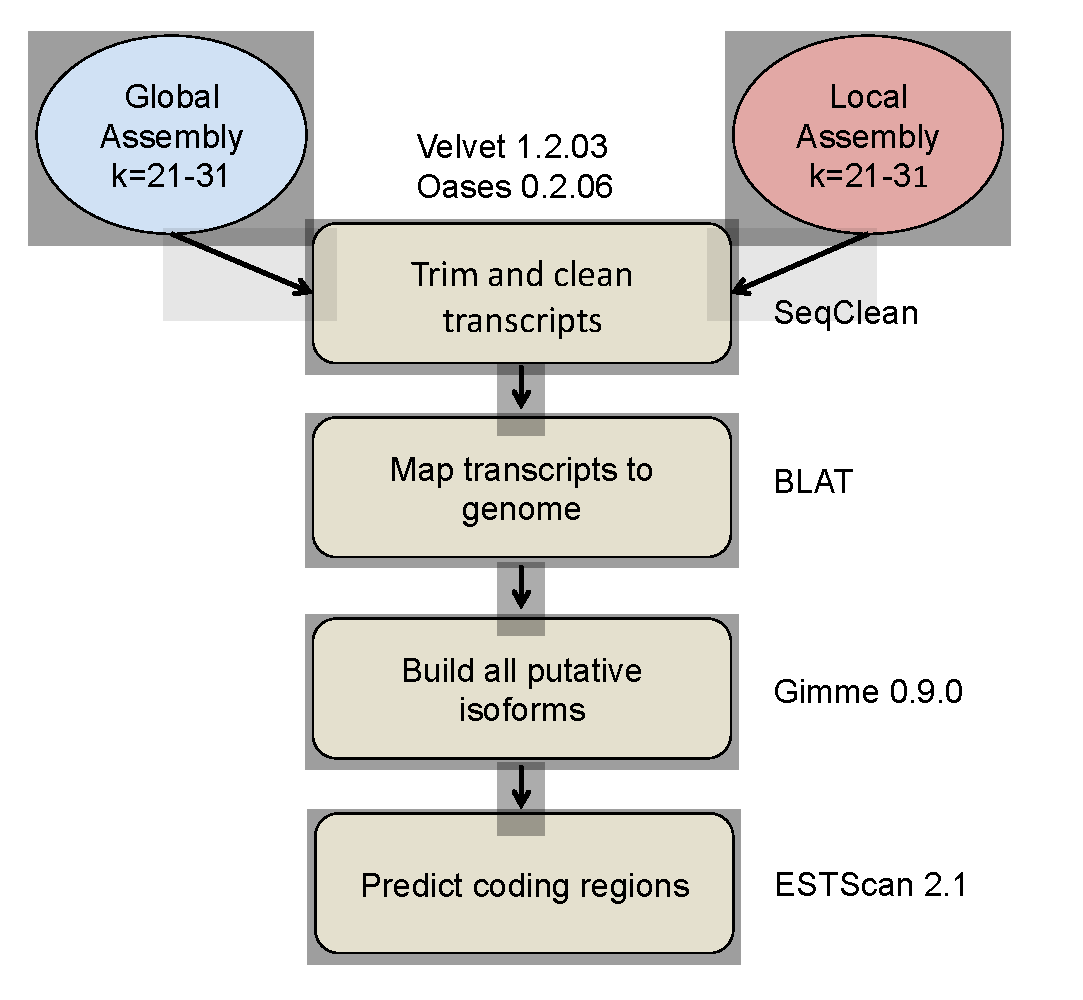
\includegraphics[width=5in]{overall_pipeline.pdf}
\end{center}
\caption{
{\bf Gene model construction pipeline.} Transcripts are obtained from two assembly methods -- global and local assembly.
Transcripts are aligned to a chicken genome by BLAT\@. Gimme then constructs gene models based on alignments of transcripts.
}
\label{overall_pipeline}
\end{figure}

\begin{figure}[!ht]
\begin{center}
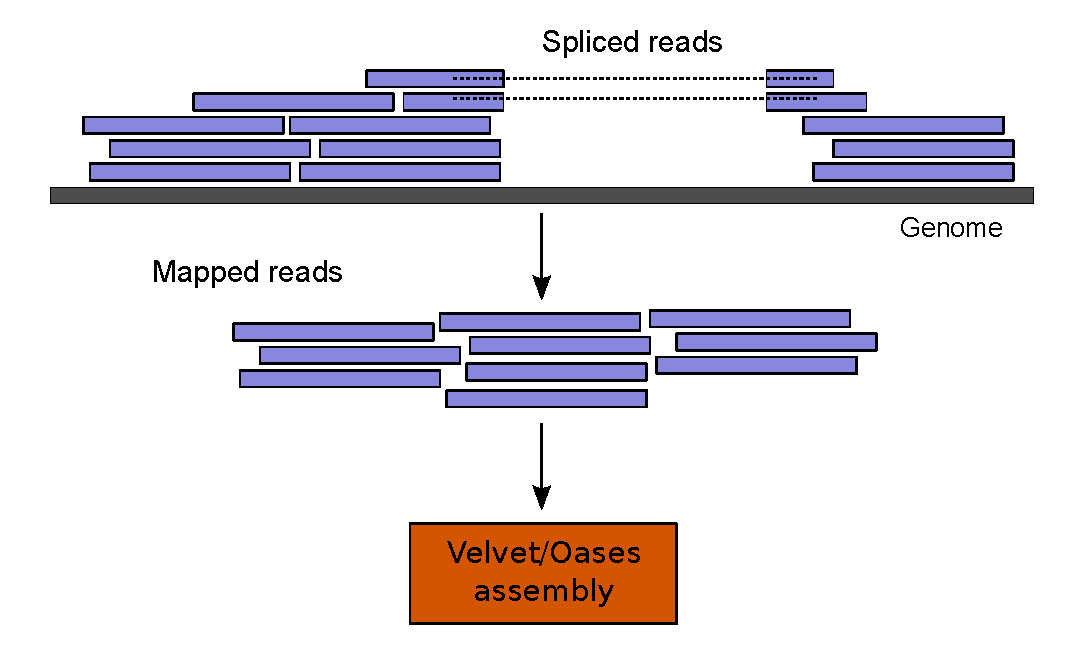
\includegraphics[width=5in]{local_assembly}
\end{center}
\caption{
{\bf Local Assembly Pipeline.}
Reads are first mapped to a chicken genome.
Then only mapped reads are assembled by Velvet and Oases.
}
\label{local_assembly}
\end{figure}

\begin{figure}[!ht]
\begin{center}
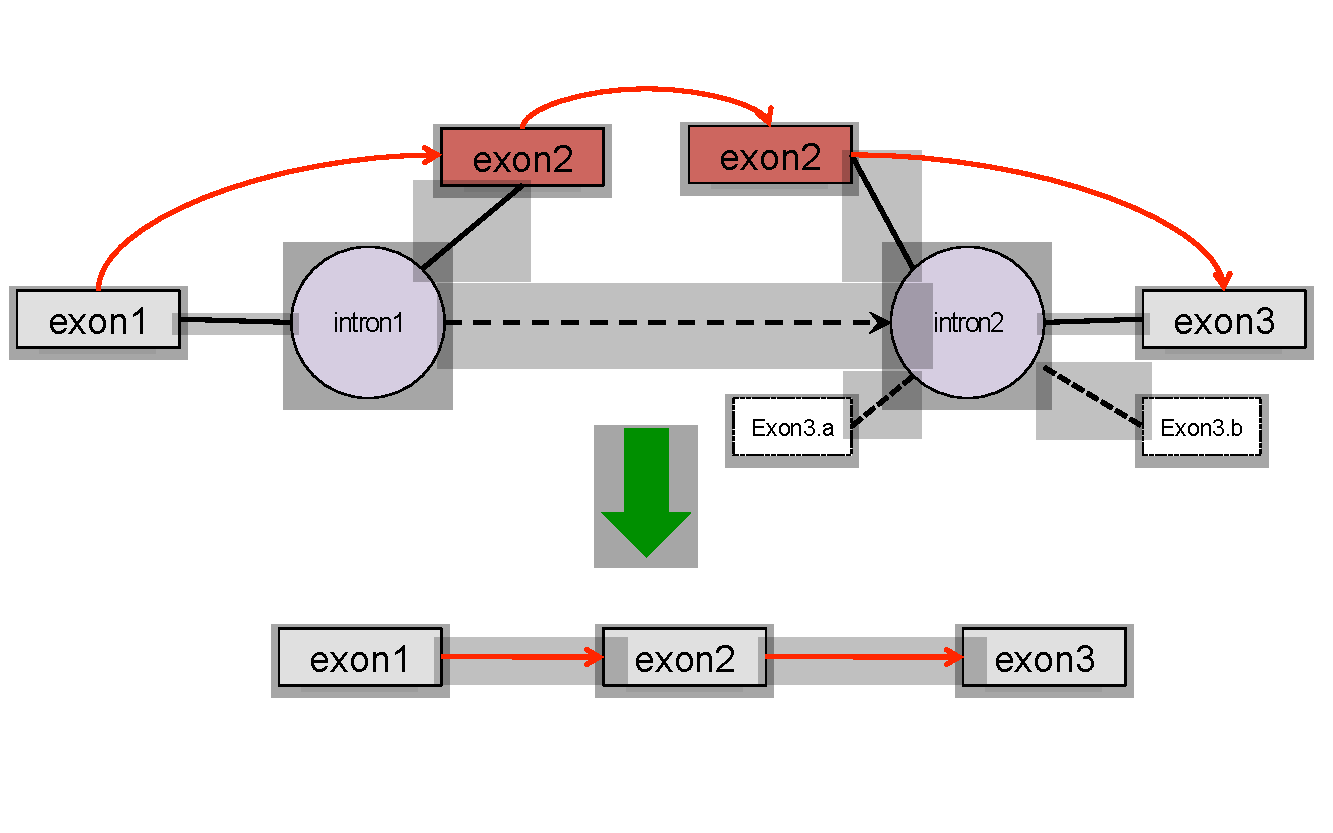
\includegraphics[width=5in]{algorithm.pdf}
\end{center}
\caption{
{\bf Intron and exon graphs.}
Each intron connects to exons whose splice junctions match it boundary.
Some exons are excluded from the final gene model if they are incomplete (exon 3a,b).
Introns sharing at least one exon are grouped together.
Then an exon graph is made using exons as nodes.
}
\label{algorithm}
\end{figure}

\begin{figure}[!ht]
\begin{center}
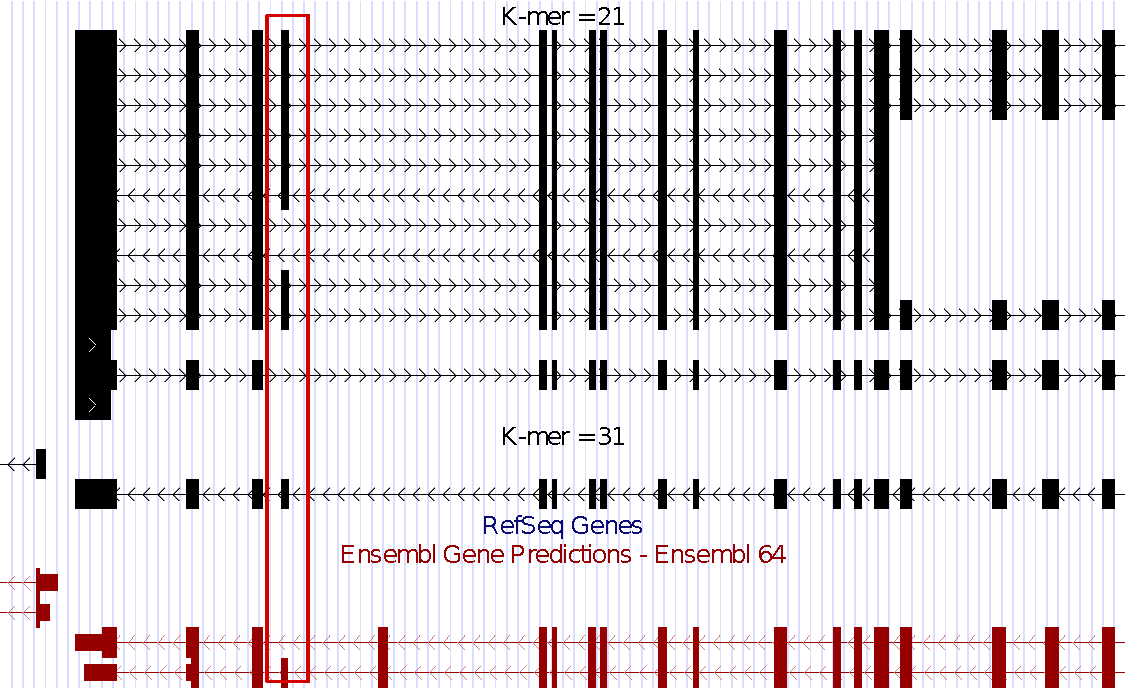
\includegraphics[width=5in]{kmers-variance.pdf}
\end{center}
\caption{
{\bf Different isoforms are detected by different k-mer lengths.}
K-mer=21 detects a skipped exon which is not detected by k-mer=31.
The skipped exon is also annotated in Ensembl gene models.
}
\label{kmer-variance}
\end{figure}

\begin{figure}[!ht]
\begin{center}
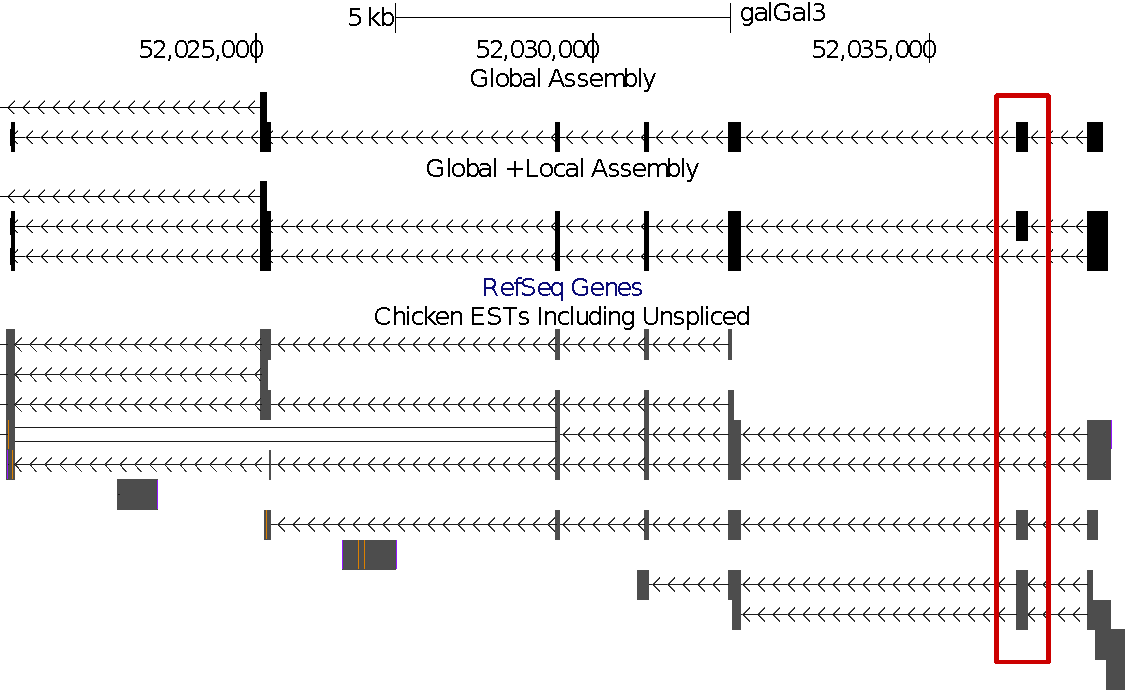
\includegraphics[width=5in]{global_vs_local.pdf}
\end{center}
\caption{
{\bf Global and local assembly detect different isoforms with the same k-mers.} 
}
\label{global_vs_local}
\end{figure}

\begin{figure}[!ht]
\begin{center}
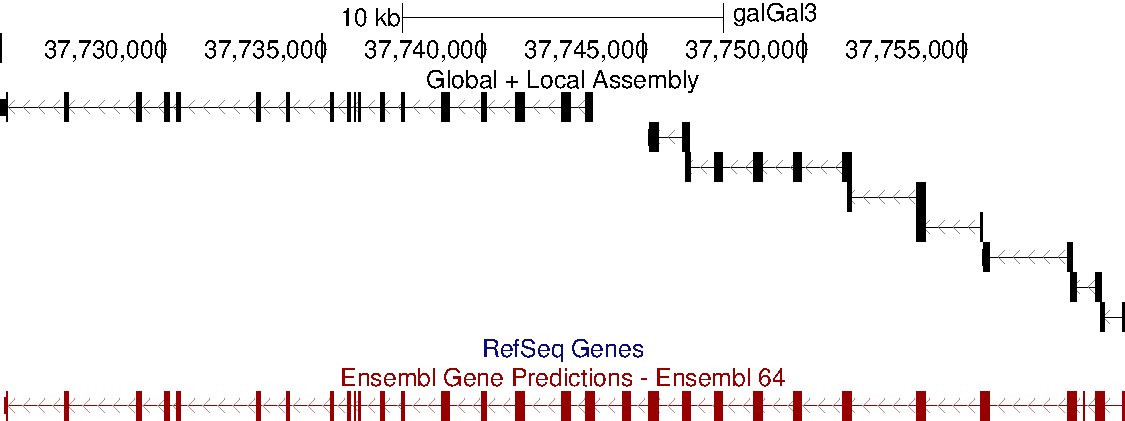
\includegraphics[width=5in]{fragmented_transcripts.pdf}
\end{center}
\caption{
{\bf Example of fragmented transcripts near $5'$ end of a long transcript.}
}
\label{fragmented_transcripts}
\end{figure}

\begin{figure}[!ht]
\begin{center}
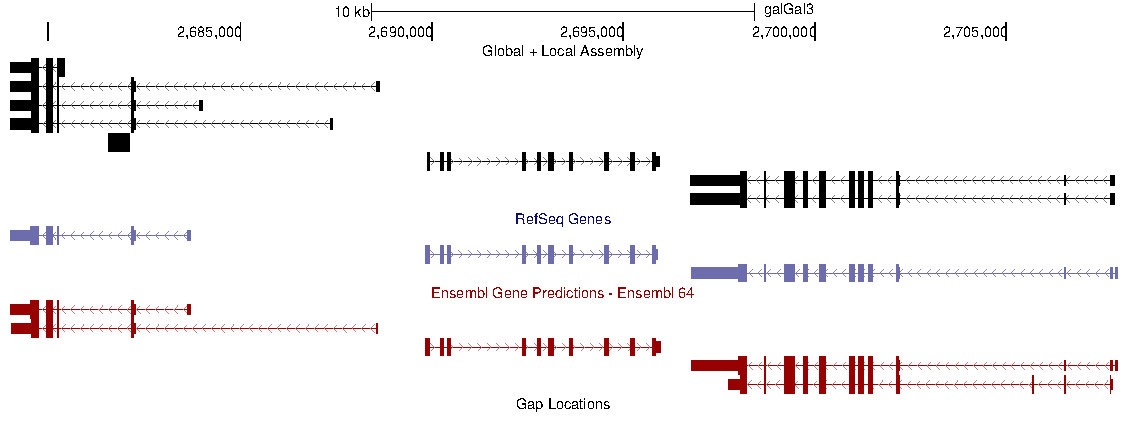
\includegraphics[width=5in]{model_comparisons.pdf}
\end{center}
\caption{
{\bf Comparison of gene models from the \emph{de novo} assembly pipeline with reference and Ensembl gene models on UCSC genome browser.}
}
\label{model_comparisons}
\end{figure}

\begin{figure}[!ht]
\begin{center}
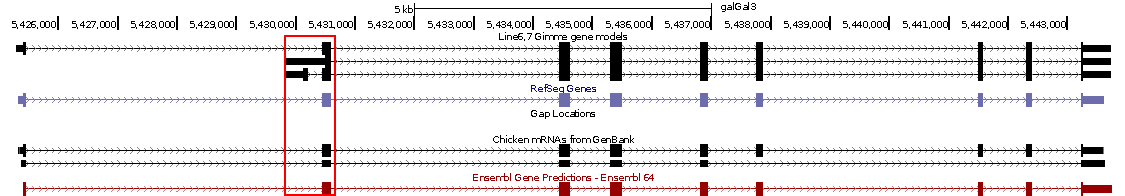
\includegraphics[width=6in]{alter_5utr.pdf}
\end{center}
\caption{
{\bf Examples of alternative $5'$ UTRs in RNA-Seq gene models.}
}
\label{alter_5utr}
\end{figure}

\begin{figure}[!ht]
\begin{center}
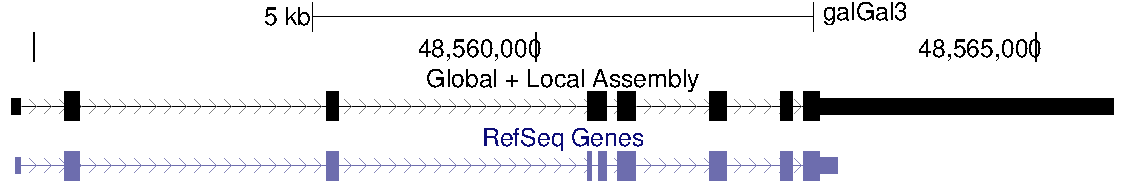
\includegraphics[width=5in]{long_utr.pdf}
\end{center}
\caption{
{\bf Examples of an extended $3'$ UTR in RNA-Seq gene models.}
}
\label{long_utr}
\end{figure}

\begin{figure}[!ht]
\begin{center}
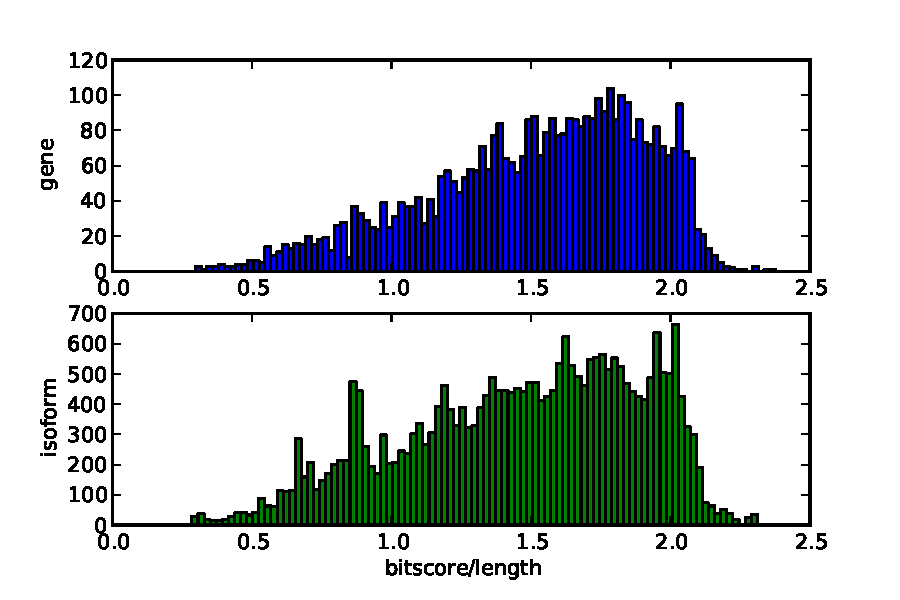
\includegraphics[width=5in]{bitscore.pdf}
\end{center}
\caption{
{\bf Histogram of bit score/length ratio of isoforms and genes that match mouse proteins.}
}
\label{bitscore}
\end{figure}

\begin{figure}[!ht]
\begin{center}
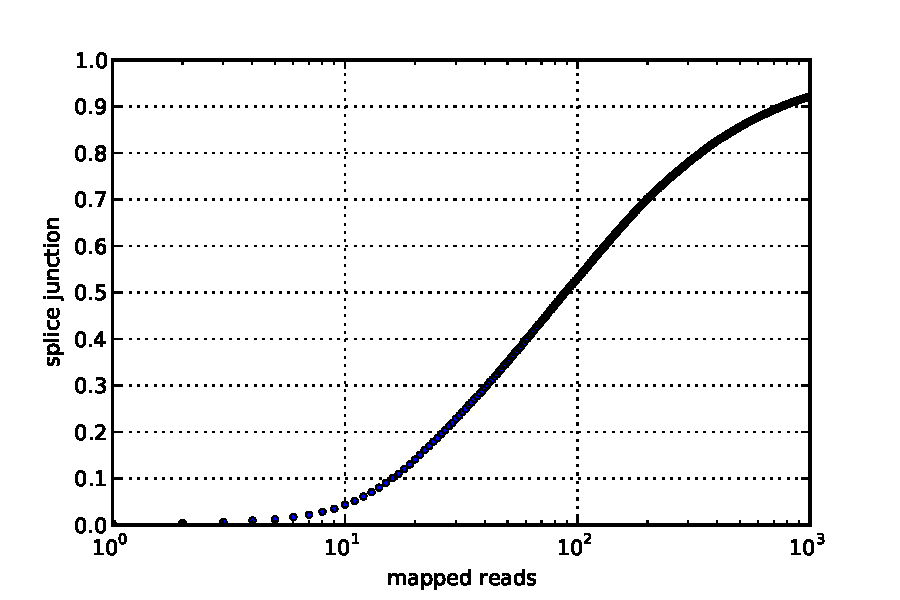
\includegraphics[width=5in]{cdf_single_splice.pdf}
\end{center}
\caption{
{\bf Cumulative counts of splice junctions with spliced reads up to 1000 reads.}
}
\label{cdf_single_splice}
\end{figure}

\begin{figure}[!ht]
\begin{center}
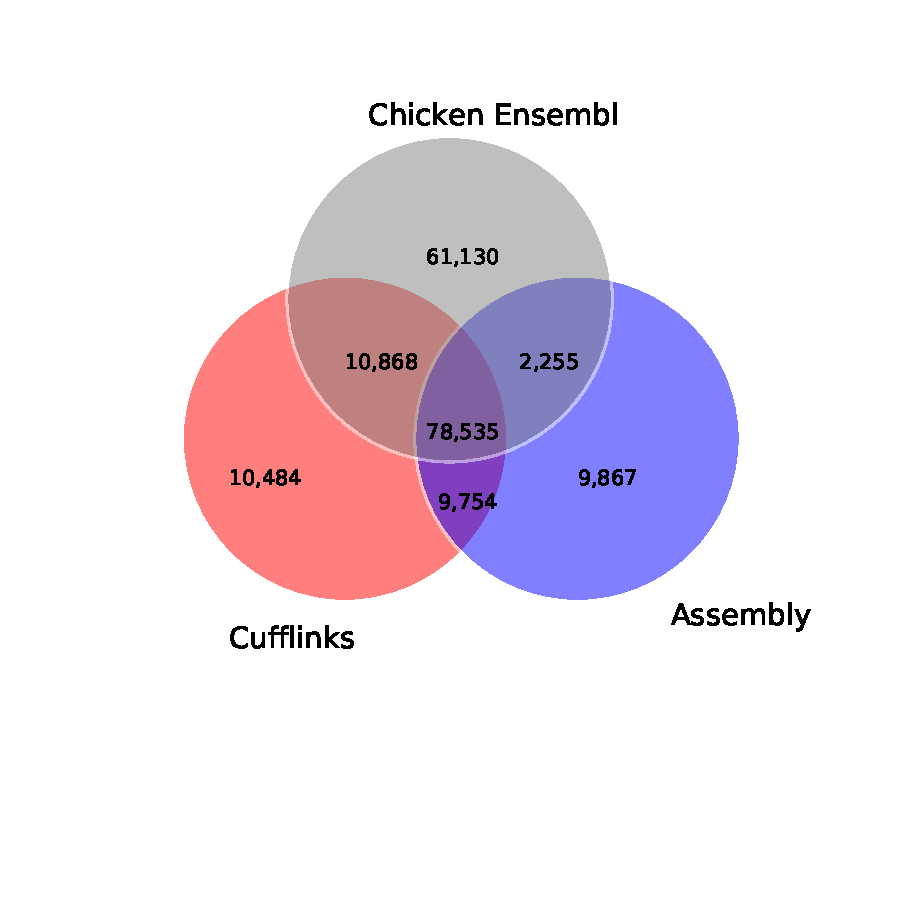
\includegraphics[width=5in]{chick_venn.pdf}
\end{center}
\caption{
{\bf Splice sites in chicken Ensembl gene models detected by Cufflinks and the \emph{de novo} assembly pipeline.}
Cufflinks detects many annotated isoforms that are not detected by the pipeline.
The figure also shows that both methods detect a large number of unannotated splice junctions, which suggests
that those junctions may be genuine.
}
\label{chick_venn}
\end{figure}

\begin{figure}[!ht]
\begin{center}
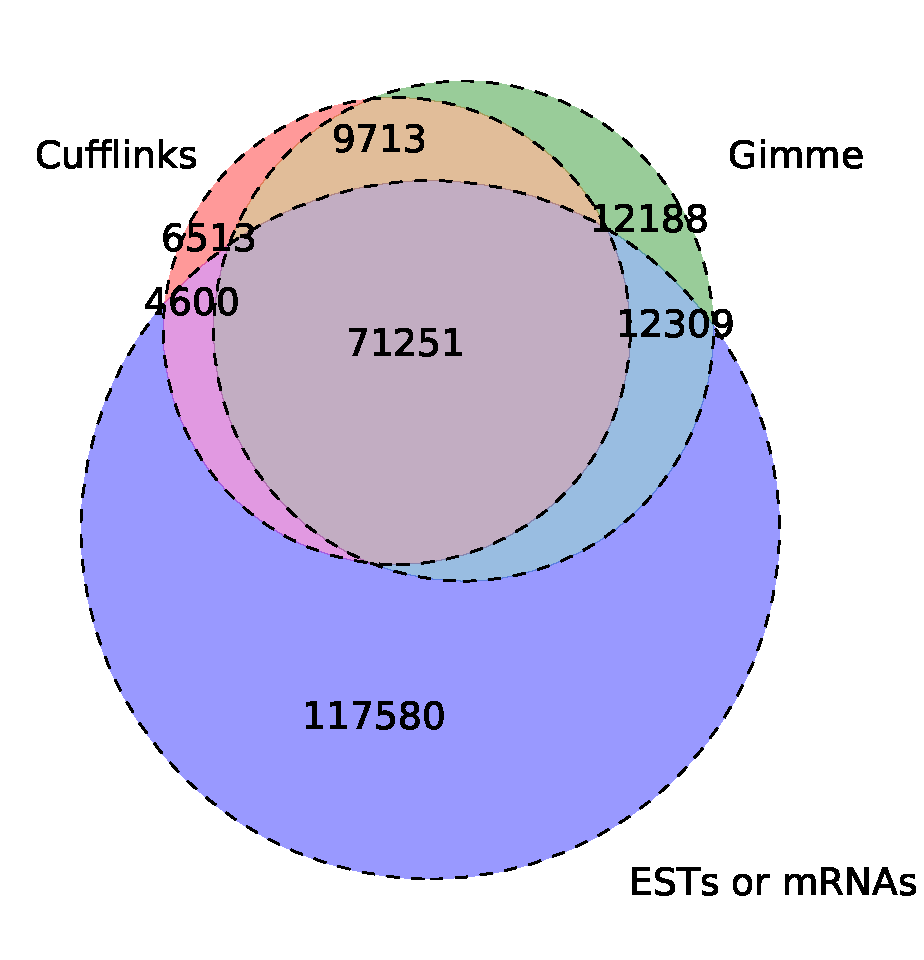
\includegraphics[width=5in]{chick_est_venn.pdf}
\end{center}
\caption{
{\bf Splice sites in Chicken ESTs detected by Cufflinks and the \emph{de novo} assembly pipeline.}
In contrast to Ensembl gene models, the pipeline and Cufflinks detects the similar number of splice junctions
from ESTs and mRNAs. This indicates that the pipeline is as efficient as Cufflinks at detecting
non-annotated splice junctions.
}
\label{chick_est_venn}
\end{figure}

\begin{figure}[!ht]
\begin{center}
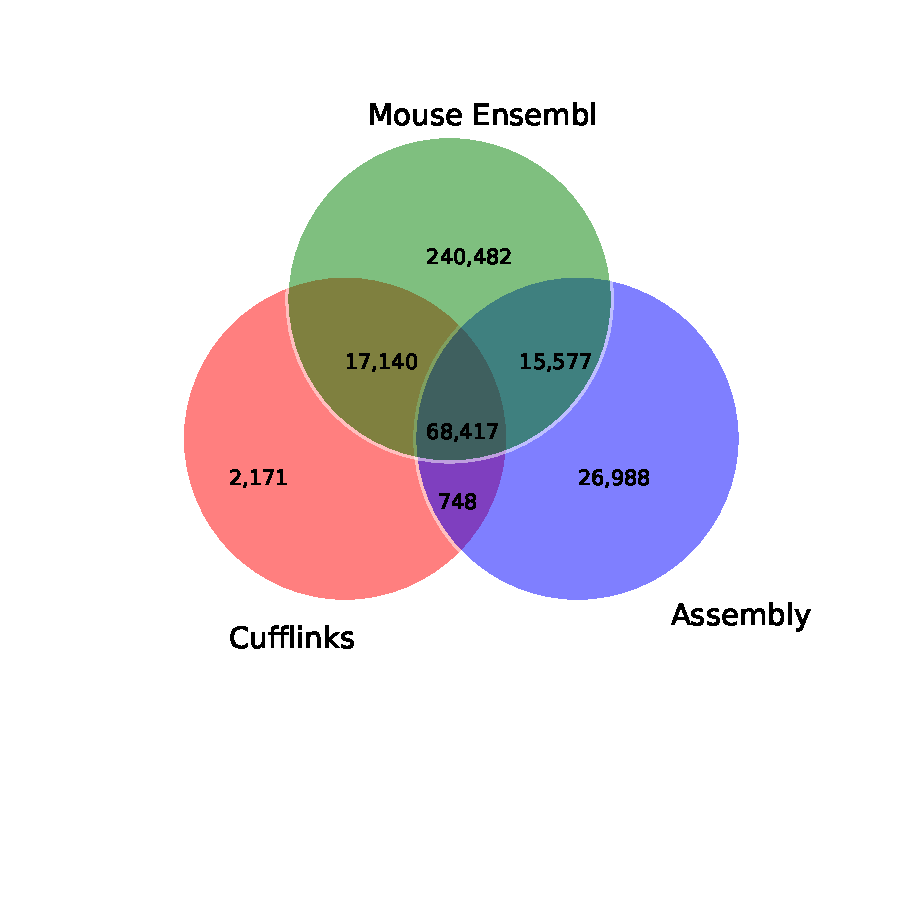
\includegraphics[width=5in]{mus_venn.pdf}
\end{center}
\caption{
{\bf Splice sites in mouse Ensembl gene models, Cufflinks and the \emph{de novo} assembly pipeline.}
In contrast to chicken datasets, Cufflinks and the pipeline detects the similar amount of non-overlapped annotated junctions.
This may due to a higher quality of gene annotations in mouse.
}
\label{mus_venn}
\end{figure}

\begin{figure}[!ht]
\begin{center}
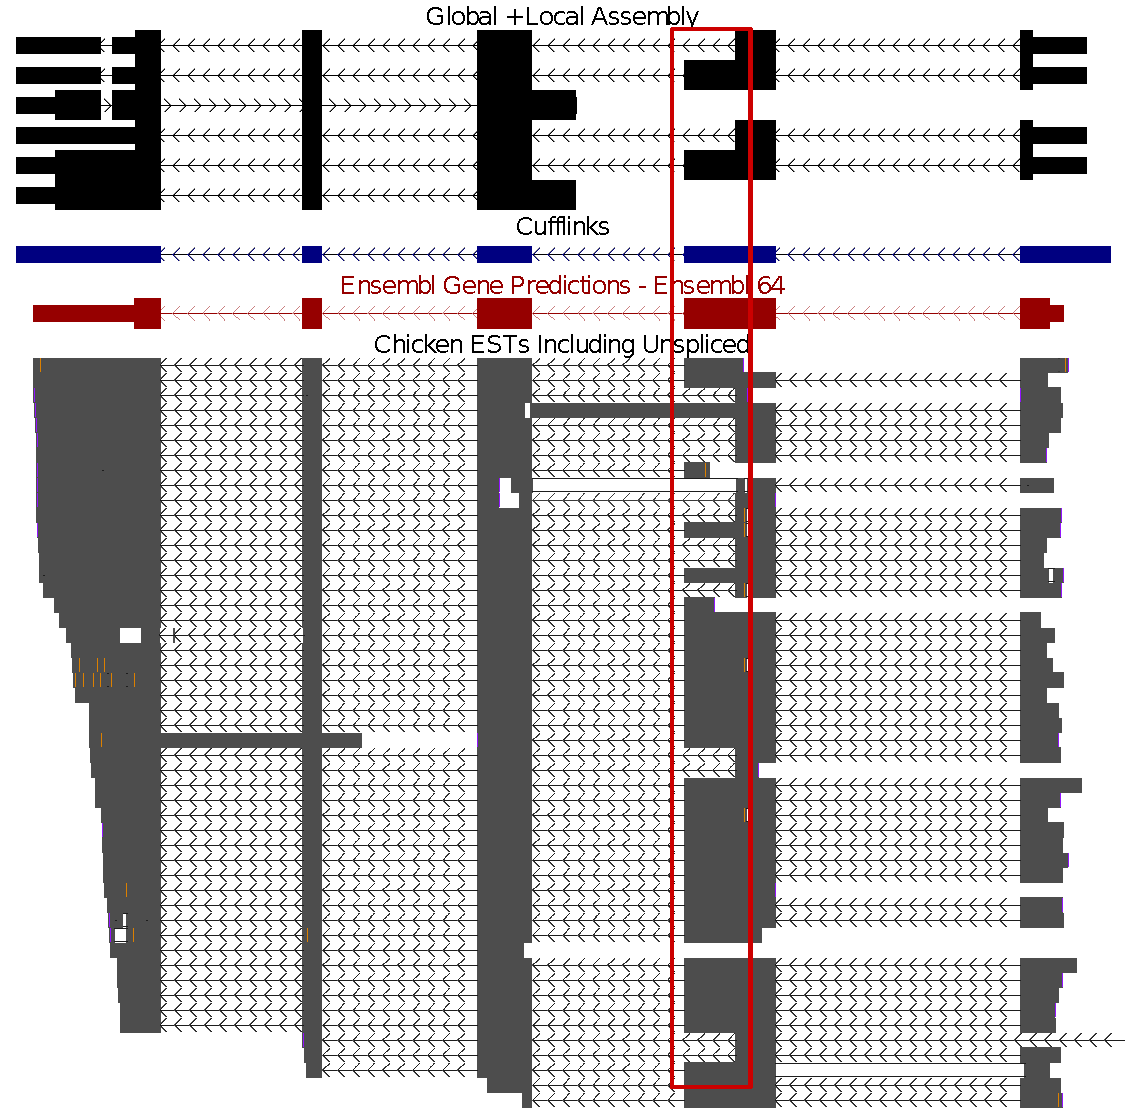
\includegraphics[width=5in]{alt_splice_site.pdf}
\end{center}
\caption{
{\bf Unannotated alternative splice site.}
The pipeline detects alternative splices site not annotated in Ensembl and Cufflinks but are supported by ESTs.
}
\label{alt_splice_site}
\end{figure}

\begin{figure}[!ht]
\begin{center}
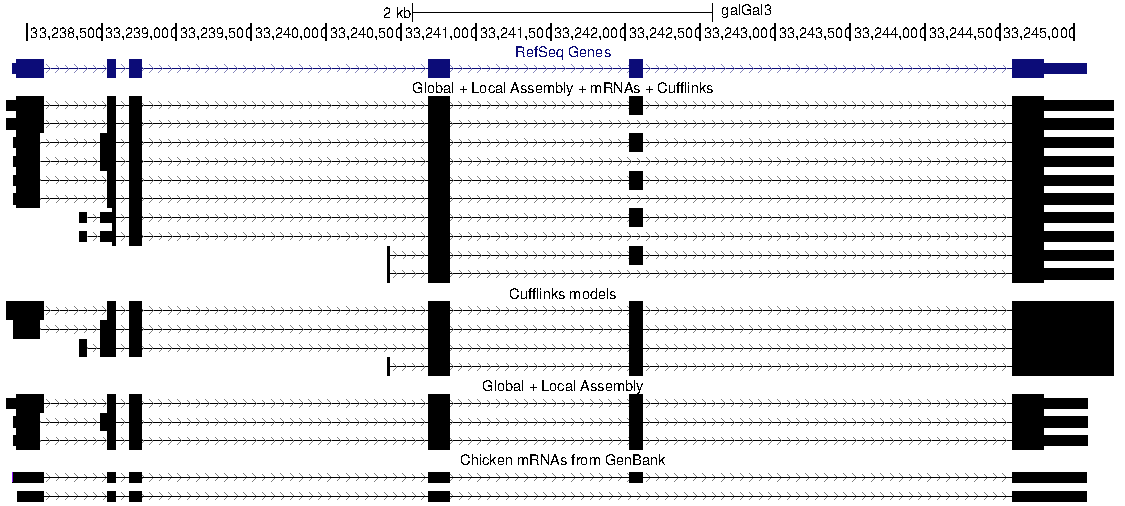
\includegraphics[width=5in]{mrna_cuff_gimme.pdf}
\end{center}
\caption{
{\bf mRNAs + Cufflinks + Assembly gene models.}
Gimme can combine transcripts from different sources to build gene models.
In this figure, the final gene model includes several isoforms not annotated in the reference gene model.
}
\label{mrna_cuff_gimme}
\end{figure}

\end{document}
